\documentclass[25pt,margin=20mm,innermargin=-6in,blockverticalspace=1mm]{tikzposter}
\geometry{paperwidth=47in,paperheight=33in}
\usepackage[utf8]{inputenc}
\usepackage{amsmath}
\usepackage{amsfonts}
\usepackage{amsthm}
\usepackage{amssymb}
\usepackage{mathrsfs}
\usepackage{graphicx}
\usepackage{caption}
\usepackage{subcaption}
\usepackage{adjustbox}
\usepackage{enumitem}
\usepackage{wrapfig}
\usepackage[backend=bibtex,style=numeric,doi=false,url=false,eprint=false,sorting=none,autocite=superscript]{biblatex}
\usepackage{bodl}
\usetikzlibrary{positioning,shapes,arrows}

\makeatletter
\def\title#1{\gdef\@title{\scalebox{\TP@titletextscale}{%
\begin{minipage}[t]{\linewidth}
\centering
#1
\par
\vspace{0.5em}
\end{minipage}%
}}}
\makeatother


\addbibresource{bibliography.bib}
\AtBeginBibliography{\footnotesize}

% set theme parameters
\tikzposterlatexaffectionproofoff
\usetheme{UofATheme}
\usecolorstyle{UofAStyle}

\title{Using Alternate References for Transcriptome Analysis of an Indigenous Australian Study Cohort}
\author{\centering \textbf{Stevie Pederson}\textsuperscript{1,2},Yassine Souilmi\textsuperscript{1,3} Hardip Patel\textsuperscript{2}, Alex Brown\textsuperscript{1,2}, Jimmy Breen\textsuperscript{1,2}}
\institute{
  \textsuperscript{1}Black Ochre Data Labs, Telethon Kids Institute
  \textsuperscript{2}John Curtin School of Medical Research, Australian National University\\
  \textsuperscript{3}School of Biological Sciences, University of Adelaide
}


% begin document
\begin{document}
\maketitle

\node [below right=28mm and 8mm] at (bottomleft |- topright) {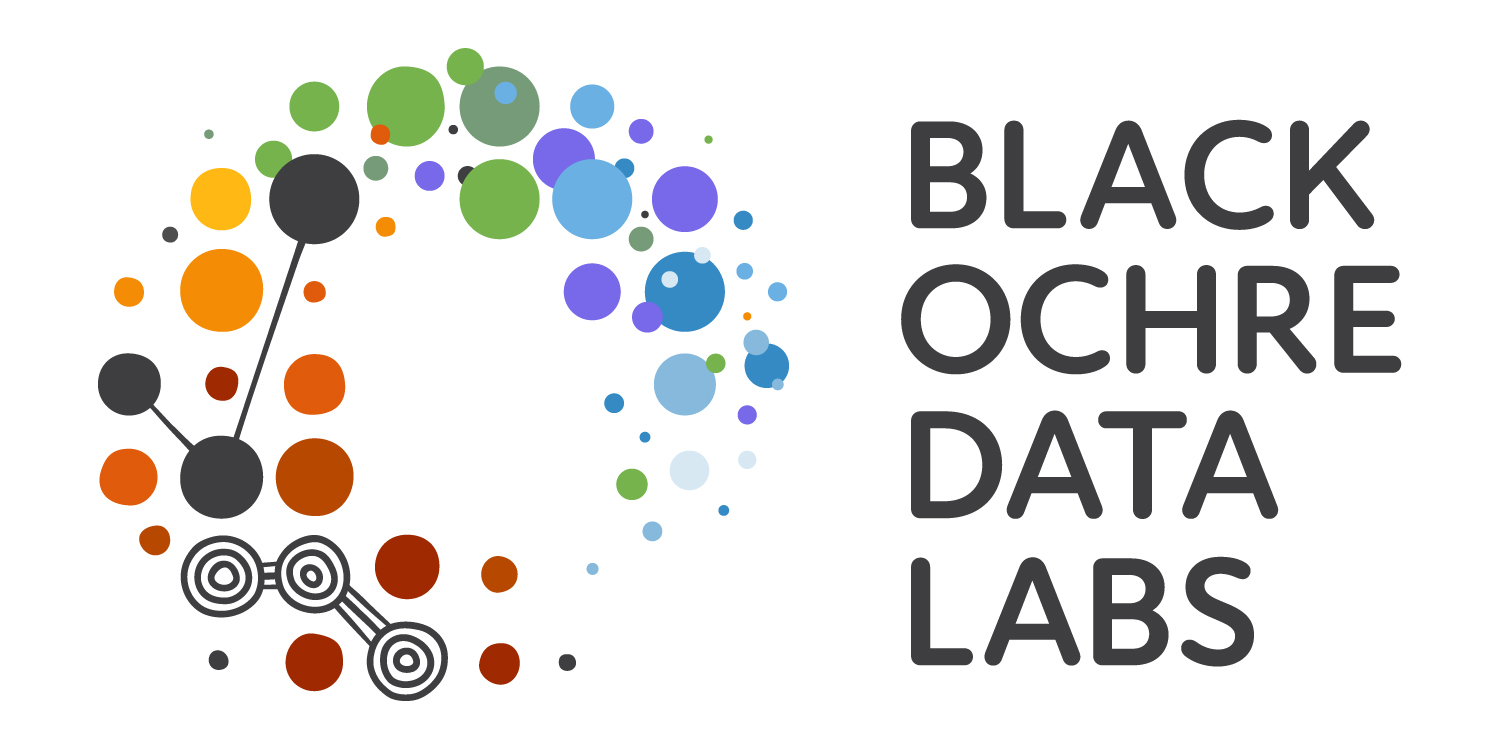
\includegraphics[width=0.12\textwidth]{bodl_logo_white_background.jpg}};
\node [below left=20mm and 10mm] at (topright) {
\includegraphics[width=0.1\textwidth]{tki.jpg}};


\centering

\block{Abstract}{
Alignment of transcriptomic data to the standard reference genome has recently been shown to be a problematic strategy\autocite{Kaminow2022-dz}. 
This is particularly relevant for populations which are poorly represented within existing repositories that capture global diversity, and when these populations themselves are known to contain a poorly characterised amount of unique variation.\\

The use of an alternate reference genome which incorporates an appropriate set of variants has also been shown to improve alignments and quantifications at the gene level. 
We propose that we will incorporate variant sets from public repositories as well as a custom set of variants identified within our study cohort and assess the impact on gene quantification across each alternate reference genome. 
This is then extended into transcript-level quantification and the incorporation of user-defined sets of variants into an alternate reference transcriptome.
In addition, a tool for creating custom reference transcriptomes has been developed.

}

\begin{columns}
    \column{0.33}
    	\block{Genomic Variability}{
		\Large
		The Indigenous Australian population contains a large amount of unique genetic diversity.
		Given that risk factors are increasingly being shown to be polygenic and dependent on the genetic background. ignoring diversity in a large cohort may limit our ability to address this contribution.\\
		
		The historical relationship between researchers and the Aboriginal community has been problematic and as such, this population is poorly represented in databases such as the 1000 Genomes Project, and the Human Genome Diversity Project.
		Prepared in a highly consultative, and indigenous-led manner, the PROPHECY study present a unique opportunity to provide access to precision medicine for members of the Indigenous Australian community.
		The unique design of the study also presents a unique opportunity to include population-level diversity across all -omics layers in the study.

    	}
    	\vspace{-1cm}
    


    \column{0.34}
    \useblockstyle{KeyBlockStyle}
    \block{The PROPHECY Study}{
    \Large
    \vspace{2mm}
    The PROPHECY study (\textbf{P}reventing \textbf{R}enal, \textbf{OP}hthalmic and \textbf{H}eart \textbf{E}vents in \textbf{C}ommunit\textbf{Y}) consists of $\sim$1400 indigenous participants drawn from regional, remote and urban locations within South Australia.
    Amongst community, the study is colloquially known as the \textit{Aboriginal Diabetes Study}.\\
    
    The PROPHECY Study is a multi-omics study including genomic variants, DNA methylation, bulk RNA-Seq, proteomics, lipidomics, metabolomics and multiple other layers, all derived from blood samples taken from the same participants.
    
    \vspace{3mm}
    }
    \useblockstyle{UofABlockStyle}

    \block{Haploid Reference Strategies}{
    Stuff

    	
    }

    \column{0.33}
    \block{Pan Genome Reference Graphs}{
		Stuff

    \coloredbox{
	    \colorlet{innerblockbodybgcolor}{white}
        \innerblock{\large \textbf{References}}{
	        \printbibliography[heading=none]
		}
	 }
	    
   }


\end{columns}
\end{document}